\section{評価及び考察}\label{sec:eval}
本章では作成したアプリケーションの検出精度や実行速度を測り、
アプリケーションの実用性を評価する。
本評価で使用するテンプレート画像及び差し替え先画像を図\ref{fig:data}に示す。
なお、適用先画像については特に言及しない限り、
本レポートに添付した「target.mp4」を使用する。
\begin{figure}[h]
    \centering
    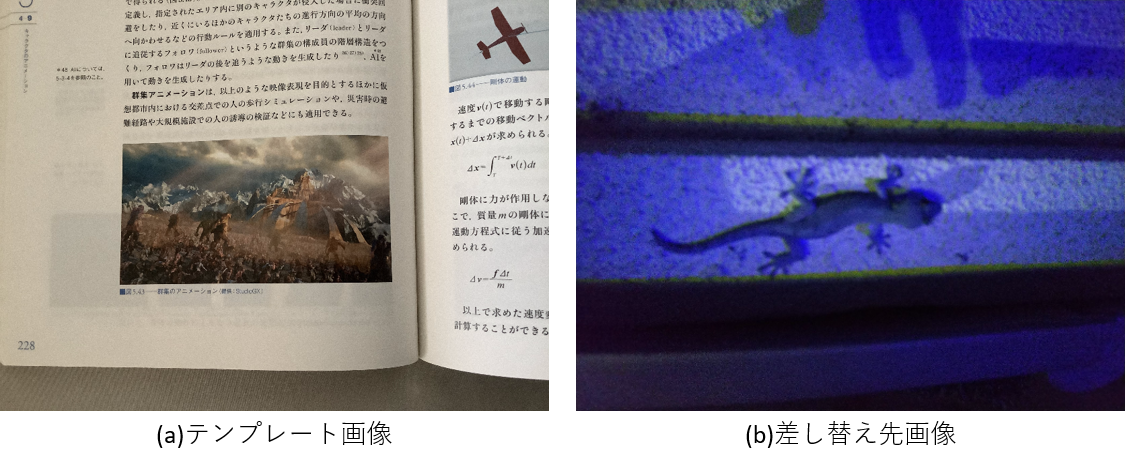
\includegraphics[width=1\linewidth]{fig/data.png}
    \caption{評価データ}
    \label{fig:data}
\end{figure}
なお、テンプレート画像については無駄な領域を省くために図\ref{fig:clip}で示されるように、
アプリケーション内でユーザが領域を選択しクリッピングしておく。
\begin{figure}[h]
    \centering
    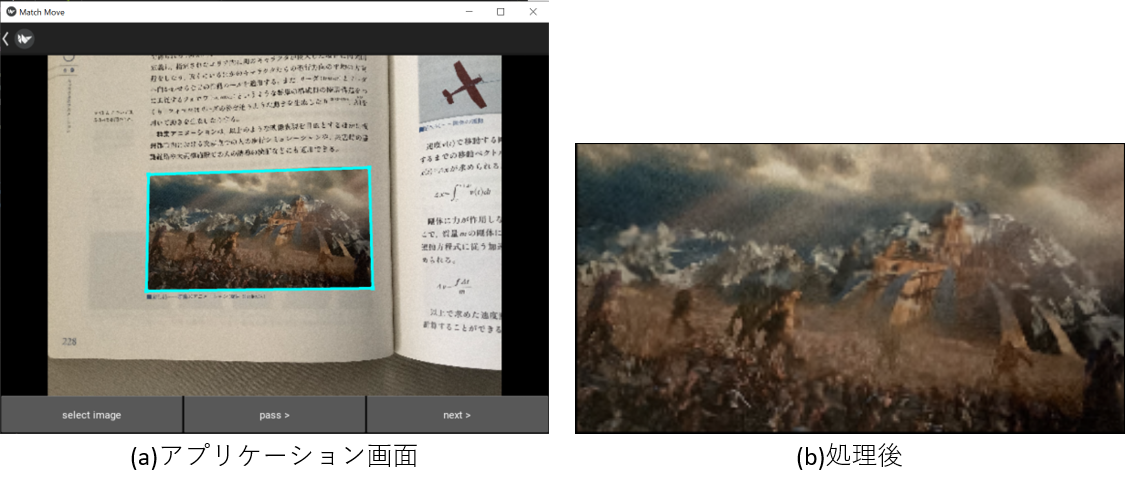
\includegraphics[width=1\linewidth]{fig/clip.png}
    \caption{テンプレート画像のクリッピング}
    \label{fig:clip}
\end{figure}
図\ref{fig:clip}(a)のアプリケーション画面において、
水色のユーザが指定したものであり、
各頂点をクリックすることで選択できるようになっている。
(b)はクリッピングした結果である。
なお変形先については\ref{sec:size}節で述べたように二種類の方法で変形する。

\subsection{ワーピング実装と速度}
本節では\ref{sec:warp}節で述べた2種類の実装の速度を比較する。
本評価では$(128, 128, 3)$の画像の適当な4点を選択し、
$(256, 256, 3)$の像の適当な4点へと変換する。
変換は複数回行い、その平均の実行時間を比較する。

表\ref{tb:warp}に線形補完及びホモグラフィ行列それぞれのアルゴリズムで実行した結果を示す。
\begin{table}[h]
    \centering
    \caption{ワーピングアルゴリズムと速度}
    \label{tb:warp}
    \begin{tabular}{lc} \hline \hline
         & 実行時間[sec]\\ \hline
        線形補完 & 0.0760 \\
        ホモグラフィ行列 & 0.0148 \\ \hline
    \end{tabular}
\end{table}
表\ref{tb:warp}からわかるように、
ホモグラフィ行列での実装は線形補完での実装と比較して
約5.14倍の速度で実行できている。
これはソースコード\ref{py:warp}
及びソースコード\ref{py:homo}のコード量から明らかである。
実際、線形補完を行うためには、点と直線の距離や、
変換のマスクなどの計算が必要であり、
テンソル計算を単純に利用しづらい。
一方でホモグラフィ行列は推定処理においてもほとんどテンソル演算に落とし込むことができるため、単純に実装でき、かつ
Numpyの特性を活かしやすい。
特にNumpyのバックエンドは低級言語で書かれており、
Pythonの素のコードより明らかに高速で処理できる。

どちら同じ結果が得られることを考えると、明らかに
ホモグラフィ行列を利用した方がよいと分かる。

\subsection{テンプレート画像のサイズと精度}\label{sec:size_acc}
本節では\ref{sec:size}節で述べた二種類のサイズとマッチングの精度を比較する。
適用先画像には「target.mp4」における1フレーム目を使用する。
また、マッチングアルゴリズムにはSIFTを使用する。
以下にそれぞれにマッチング処理を適用した結果を
図\ref{fig:size_acc_same}及び\ref{fig:size_acc_diff}に示す。

\begin{figure}[h]
    \centering
    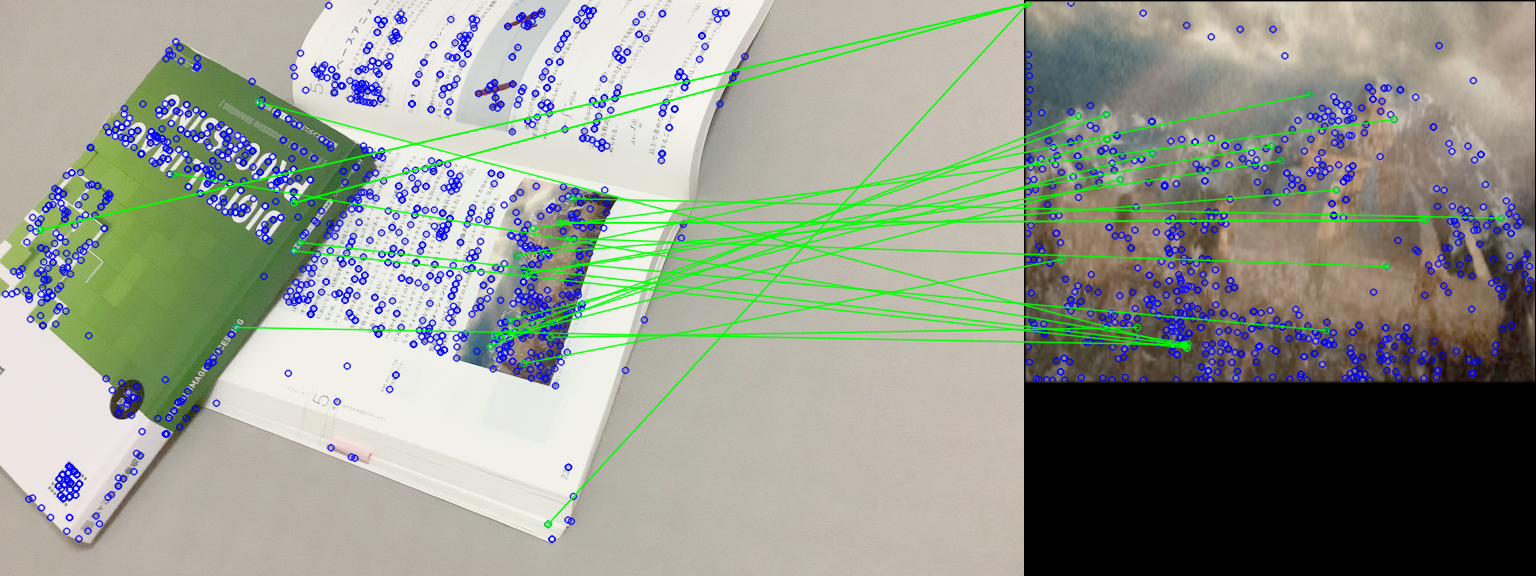
\includegraphics[width=1\linewidth]{fig/matches_SIFT_difference.png}
    \caption{差し替え先画像の高さ・幅に合わせるマッチング}
    \label{fig:size_acc_diff}
\end{figure}

\begin{figure}[h]
    \centering
    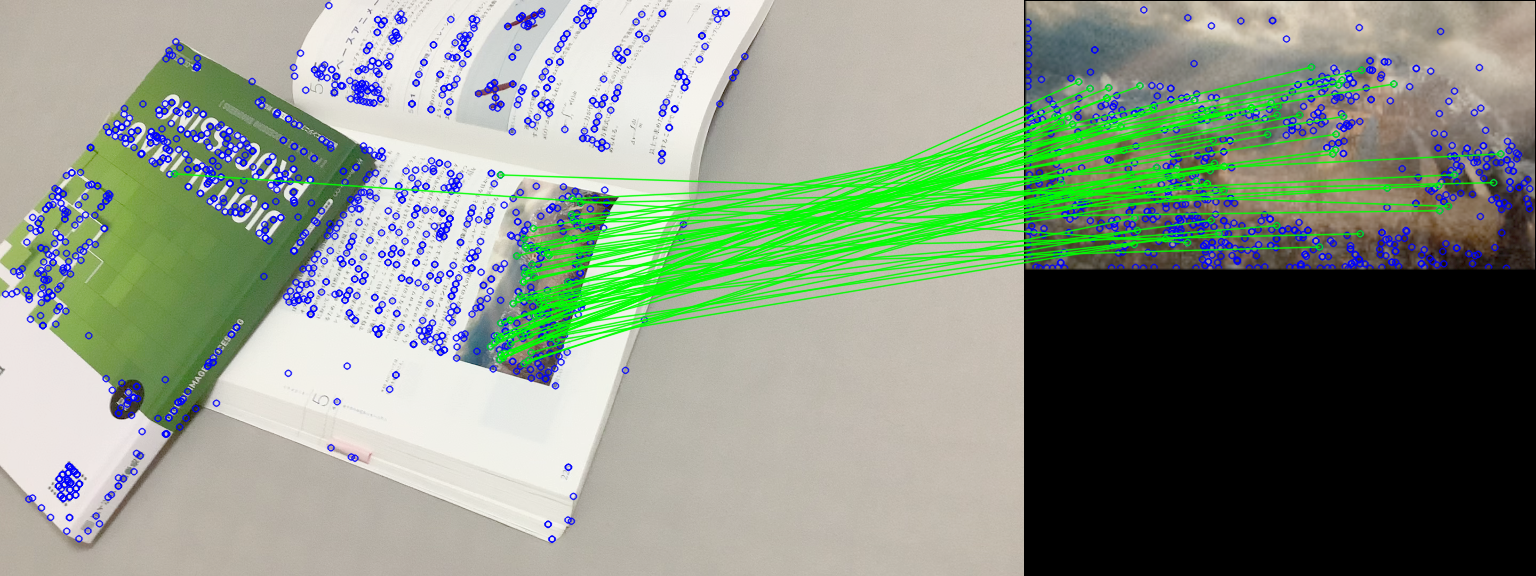
\includegraphics[width=1\linewidth]{fig/matches_SIFT_same.png}
    \caption{テンプレート画像の高さ・幅に合わせるマッチング}
    \label{fig:size_acc_same}
\end{figure}

図\ref{fig:size_acc_same}及び\ref{fig:size_acc_diff}から分かるように、
アスペクト比を変化させないほうが明らかに検出精度が高いことが分かる。
この図から、マッチング数、ミスマッチ数を数えた結果を表\ref{tb:size_acc}に示す。
なお、ミスマッチ数については正確に数えることが困難であるため、
明らかに適用画像から外れた点のみを数えた。

\begin{table}[h]
    \centering
    \caption{テンプレート画像のサイズと精度}
    \label{tb:size_acc}
    \begin{tabular}{lccc} \hline \hline
         & マッチング数 & ミスマッチ数 & 精度[\%]\\ \hline
        差し替え先画像の高さ・幅に合わせる & 28 & 8 & 71.4 \\
        テンプレート画像の高さ・幅に合わせる & 68 & 2 & 97.1 \\ \hline
    \end{tabular}
\end{table}

表\ref{tb:size_acc}から分かるように、
マッチング数においてもミスマッチ数においても
テンプレート画像の高さ・幅に合わせた方が優れている。
結果として後者の方が高い精度を記録している。

この結果を踏まえて、以降の評価ではテンプレート画像の高さ・幅に画像サイズを合わせて行う。

\subsection{置換精度}
本節では、様々な状況における置換の精度を評価する。
具体的には図\ref{fig:env_data}に示す、
通常の画像、ブレの画像、斜めから見た画像、そして90°の回転を与えた画像
に対して正しく置換できるかを評価する。

\begin{figure}[h]
    \centering
    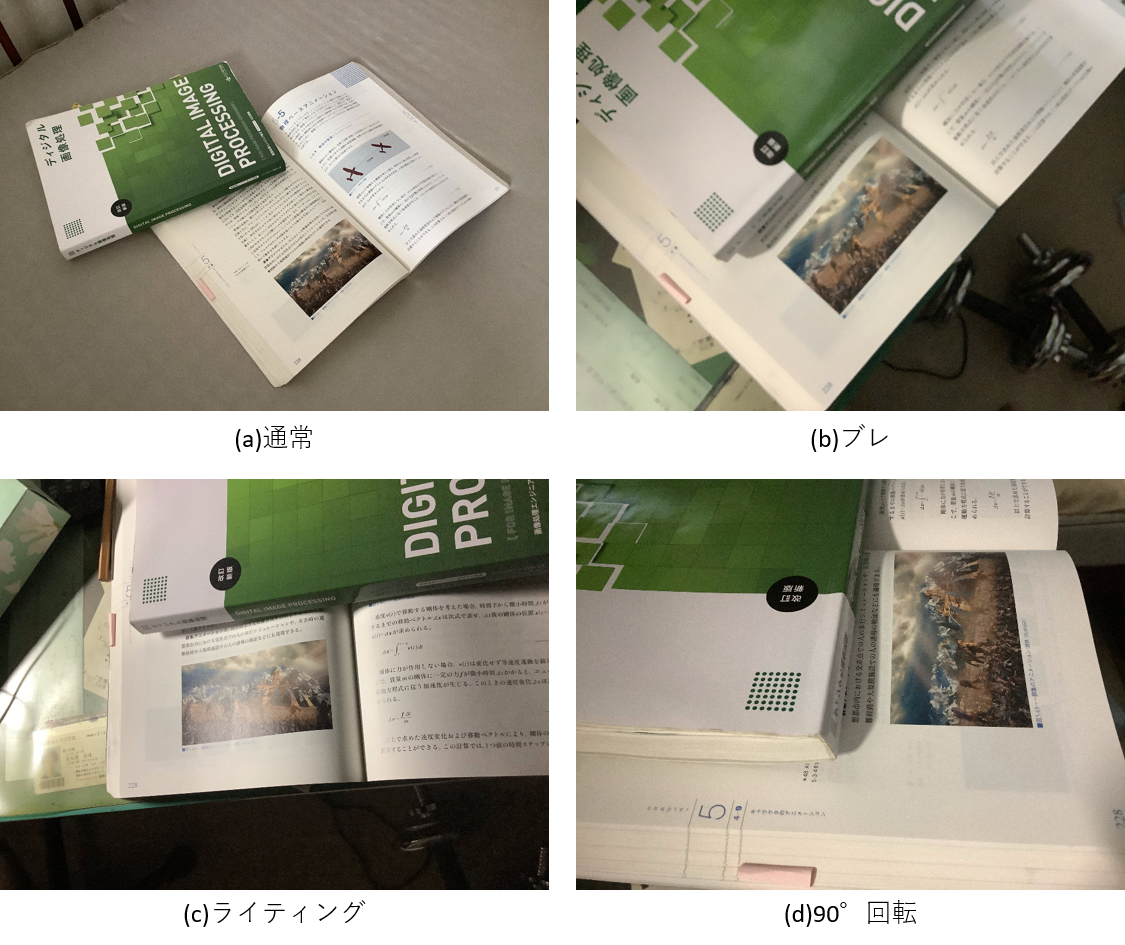
\includegraphics[width=1\linewidth]{fig/env_data.png}
    \caption{環境の異なる各データ}
    \label{fig:env_data}
\end{figure}

この評価は数値で数値で表すことが難しいため、視覚的に比較する。
図\ref{fig:various_env}に実行結果を示す。
\begin{figure}[h]
    \centering
    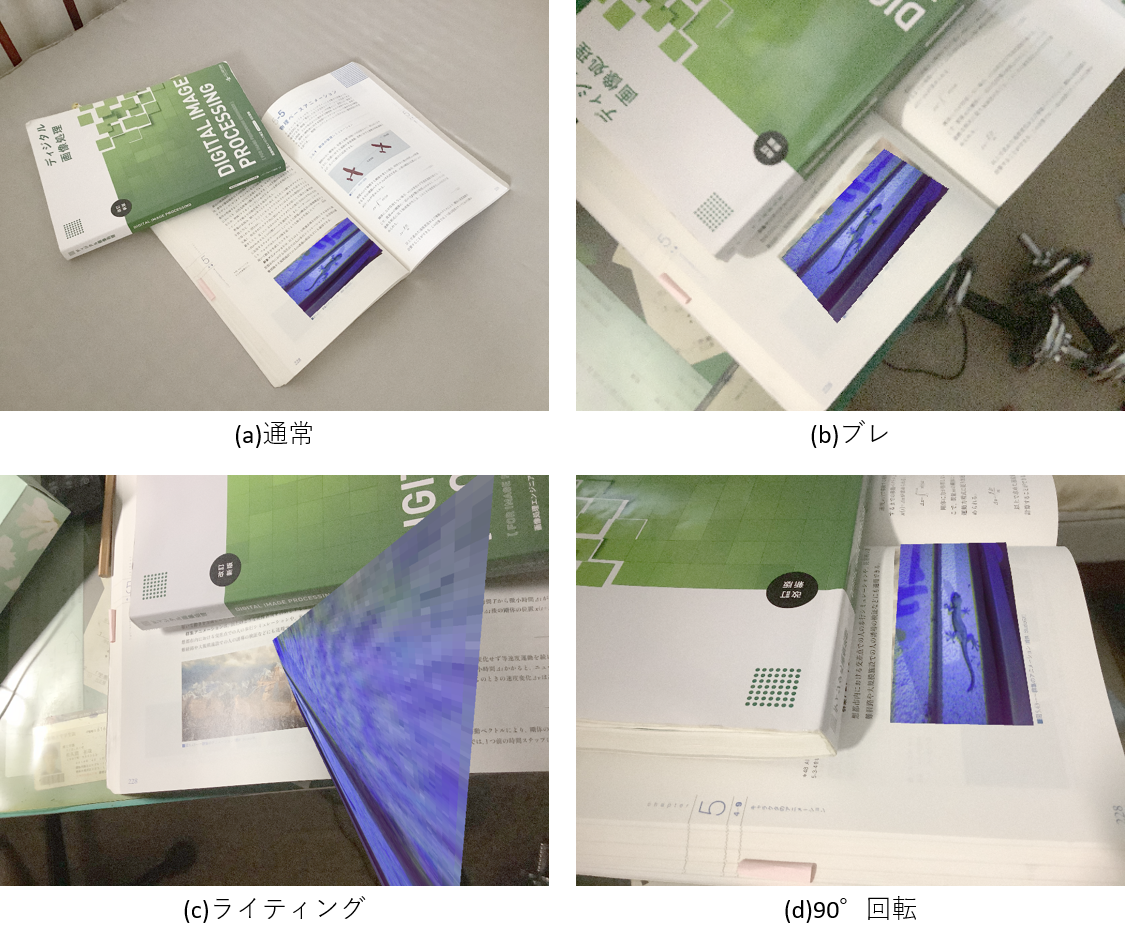
\includegraphics[width=1\linewidth]{fig/env.png}
    \caption{各環境下での置換結果}
    \label{fig:various_env}
\end{figure}
図\ref{fig:various_env}(a)(b)(d)から分かるように、多少のブレや回転に対しては、
ある程度頑健に作用している
また、(a)(b)(d)はどの画像もスケールが異なっているのにもかかわらず、
置換できていることからスケールに対しても頑健であることが分かる。
これは本アプリケーションが特徴量検出アルゴリズムとしてSIFTを採用していることに起因している。
SIFT特徴量はスケールや移動、回転に対して頑健な性質をもつ。
そのために(a)や(d)において問題なくマッチングを行い、置換できたと言える。
また、今回発生したブレは等方向的あることから、
ある種のスケールと捉えられるため、SIFTで上手くマッチングできたと考えられる。
一方で(c)のようにライティングが
変化した際には上手く置換できていないことが分かる。
これは、今回与えたライティングは対象領域を不均一に変化させていることが原因であると
考えらえる。これは画像のテクスチャが変化していることを意味するため、
正しくマッチングを行えなかったと考えられる。

\subsection{部分領域抽出による精度及び速度向上}
本節では\ref{sec:acc_speed}で説明した手法によって、
動画データに対して、精度向上及び速度向上を達成できたかを評価する。
本評価においてソースコード\ref{py:replace2}のradiusは0とした。

表\ref{tb:apply_time}に1フレーム当たりの実行時間を示す。
なお、この評価にはフレームの読み出しから、
置換結果の書き込みまでを含めた全体の時間である。
\begin{table}[h]
    \centering
    \caption{テンプレート画像のサイズと精度}
    \label{tb:apply_time}
    \begin{tabular}{lccc} \hline \hline
         & 実行時間[sec/frame] \\ \hline
        適用前 & 0.287 \\
        適用後 &  0.243 \\ \hline
    \end{tabular}
\end{table}
表\ref{tb:apply_time}から分かるようにアルゴリズムを適用することで、
1フレーム当たりの実行時間は約84.7\%になっている。
本評価で使用した動画は全体で131フレームあるため、
処理時間は5.76秒だけ削減することができた。
アルゴリズムを適用することによって探索領域は約40\%になっており、
その分だけ計算が削減されるが、
実行時間のはそれほど減少しないのは、領域を切り出すために、
ソースコード\ref{py:replace2}の36から48行目のような処理を行う必要があるためであると
考えられる。

精度向上に関しては添付した「result\_before.mp4」「result\_after.mp4」を参照されたい。
精度に関しては一長一短であるように見られる。
適用前の「result\_before.mp4」においては、前半はより安定しているが、
後半にカメラの移動が速くなると、上手く検出できなくなっている一方で、
「result\_after.mp4」は前半の安定感こそ多少劣るものの、
後半の誤差は比較的小さいように思われる。
特に結果が顕著であったフレームを図\ref{fig:apply}に実行結果を示す。

\begin{figure}[h]
    \centering
    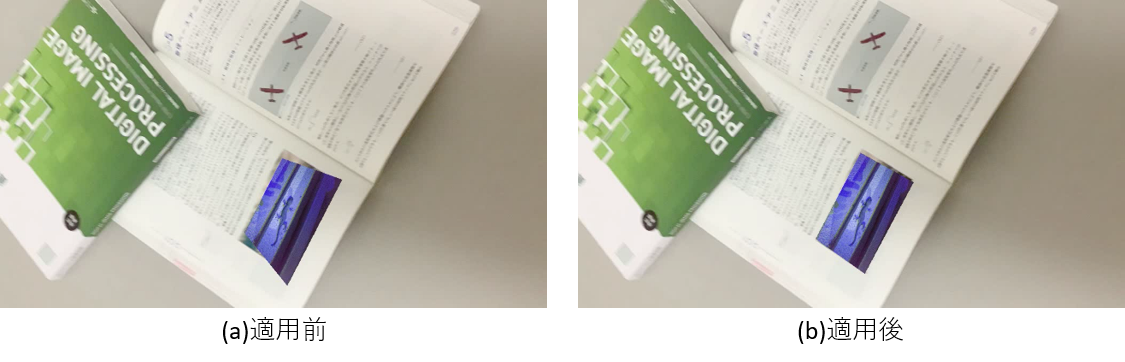
\includegraphics[width=1\linewidth]{fig/apply.png}
    \caption{適用前後で変化が顕著であったフレーム}
    \label{fig:apply}
\end{figure}

図から分かるようにこのフレームは素早くカメラを移動したことにより、
ある方向にブレが生じている。
これによって、適用前の結果では本来対応しているはずの画素同士の類似度が低下し、
誤った対応をとってしまったためであると考えらえる。
適用後の場合は探索領域を絞ったために誤った対応をとる確率が低下し、
比較的上手く置換できたと言える。


% \begin{table}[h]
%     \centering
%     \caption{テンプレート画像のサイズと精度}
%     \label{tb:size_acc}
%     \begin{tabular}{lccc} \hline \hline
%              & target & light
%         通常 & 3.035+106.429+99.911+12.75595792652888
%     \end{tabular}
% \end{table}